\documentclass[11pt, a4paper, twoside, titlepage ,dvipsnames]{report}
\usepackage[a4paper, margin=3cm]{geometry}
\usepackage[section]{placeins}
\usepackage[utf8]{inputenc}
\usepackage{amsfonts, amsmath, amssymb}
\usepackage{physics}
\usepackage{tikz}
\usepackage{float}
\usepackage{graphicx}
\usepackage[style=numeric-comp, sorting=none]{biblatex}

\usepackage[format=plain, font=footnotesize]{caption}
\usepackage[format=plain, font=footnotesize]{subcaption}

\usetikzlibrary{shapes.arrows, fadings, positioning}

\addbibresource{ref.bib}
\renewcommand*{\bibfont}{\footnotesize}
% \pagenumbering{gobble}

\begin{document}

\begingroup
    \centering
    \Large Quasilinear Time Decoding Algorithm for \\Topological Codes with High Error Threshold\\[.5em]
    \large Mark Shui Hu\footnote{S.Hu-1@student.tudelft.nl}, David Elkouss\par
\endgroup
\vspace{2em}
One of the most promising approaches for fault-tolerant quantum computation is based on surface quantum error correcting codes \cite{dennis2002topological, kitaev2003fault}. With surface codes, error correction only requires the measurement of local operators on a 2-dimensional lattice of qubits. The measurement outcome, called the syndrome, is passed to the decoding algorithm to deduct the error that has occurred and to supply a correction operator. 
%It is crucial for a decoder to perform fast, where any speed-up of the decoder leads to a reduction of the noise strength as a decreased time between two rounds of correction induces the appearance of fewer errors, and the decoder must be able to keep pace with the clock-speed of the quantum computer.
The resilience against errors can be improved by increasing the system size whilst the physical error rate is below a threshold value $p_{th}$. For this, it is essential that the decoder has low time complexity; if the clock-rate of the quantum computer becomes limited by the decoder, the advantages of increasing the system size could be compromised.

Arguably, the most popular decoder for surface codes is the Minimum-Weight Perfect Matching (MWPM) decoder \cite{dennis2002topological}. The basic principle behind this approach is to identify the \emph{lowest weight} error configuration that can produce the syndrome. In general this is a good approximation to the optimal maximum likelihood decoder \cite{bravyi2014efficient}. For a toric code that only suffers random Pauli noise, the optimal code threshold is $p_{th} = 10.9\%$, whereas the MWPM decoder has $p_{th} = 10.3\%$. The MWPM matchings are found by constructing a fully connected graph between nodes of the syndrome, which leads to a cubic worst-case time complexity of $\mathcal{O}(n^3)$ \cite{kolmogorov2009blossom}.

Many other decoding algorithms have been developed \cites{fowler2013minimum, duclos2013fault, hutter2015improved, watson2015fast, tuckett2018ultrahigh, kubica2019cellular, torlai2017neural, varsamopoulos2017decoding}. Here, we build on top of a recently proposed decoder called the Union-Find (UF) decoder. It combines a very low time complexity with a high threshold \cite{delfosse2017linear, delfosse2017almost} making it a practical solution for real devices. 
The UF decoder maps each syndrome to a vertex in a non-connected graph on the code lattice, and grows clusters of vertices locally by adding iteratively a layer of edges and vertices to existing clusters until 
all clusters have an even number of non-trivial syndrome vertices. It then trims the clusters until all non-trivial syndrome vertices are paired and linked by a path, which is the correcting operator. 
By growing the clusters of vertices in order of their sizes, the UF-decoder can be regarded as a heuristic for minimum-weight matching, and has a threshold of $p_{th} = 9.9\%$ for the toric code. 
The complexity of the UF decoder is driven by the merging between clusters. For this the algorithm uses the Union-Find or disjoint-set data structure \cite{tarjan1975efficiency}, which has worst-cast time complexity $\mathcal{O}(n\alpha(n))$, where $\alpha$ is the inverse of Ackermann's function. For any physical feasible amount of qubits, this value is $\alpha(n) \leq 3$, leading to an "almost-linear" time complexity.

%While the time complexity of the UF decoder is impressive, its error threshold has prevented its rise in popularity in the realm of decoding algorithms. Even with the discrepancy of just $0.4\%$ compared to MWPM, it is the latter that most other works use for fidelity and comparison with their own works. 
\textbf{We propose here a modification of the UF decoder that improves the heuristic for minimum-weight matchings. The modified decoder, which we dub the \emph{Union-Find Balanced Bloom decoder} (UFBB), achieves near MWPM thresholds while retaining a quasilinear time complexity.}

In the following we give some intuition into how the UFBB decoder works. Consider the cluster of vertices $\mathcal{V}=\{v_0,v_1,v_2\}$ in Figure \ref{fig1}. Now let us investigate the weights of a matching if an additional vertex $v'$ is connected to the cluster. 
If $v'$ is connected to $v_0$ or to $v_2$, then the resulting matchings have a total weight of 2: $(v',v_0)$ and $(v_1,v_2)$, or $(v_0,v_1)$ and $(v_2,v')$. However if $v'$ is connected to vertex $v_2$, then the total weight is 3: $(v', v_1)$ and $(v_0, v_2)$. Inspired by this idea, we introduce the concept of potential matching weight (PMW) of a vertex. 

The calculation of the PMW requires to introduce a new data structure that we call the node set of a cluster. The node set of a cluster is a partition of the cluster such that each element of the partition consists of a set of adjacent vertices that are either interior elements in the associated graph or have equal PMW (Figure \ref{fig2}). The calculation of the PMW is performed by two depth-first searches of the node set (Figure \ref{fig3}), where the PMW is translated into a node delay that determines the priority for cluster growth, such that the growth of a cluster moves towards equal PMW in the cluster (Balanced Bloom).
%The decoder follows the heuristic of 1) growing first smaller clusters (UF) and 2) growing first vertices with zero delay to minimize the weight of the matchings (BB). 

The UFBB decoder has a higher complexity than the UF decoder. Due to the merges of clusters, the PMW values in a cluster change and need to be recalculated, which in turn requires to join the associated node sets. These join operations are more complex than those of the UF (union of vertex sets). However, we can show that the worst-case time complexity of UFBB is $\mathcal{O}(n \log n)$, which is still quasilinear.

Our numerical results show that the error threshold of the UFBB decoder (Figure \ref{fig4}) is $p_{th} = 10.25\%$ compared to $10.02\%$ for our implementation of the UF decoder and near the threshold of MWPM $10.35\%$ (thresholds differ from reported value due to changes in cluster sorting, fitting parameters, etc.). Including measurement errors, the UFBB decoder achieves a threshold of $2.86\%$, compared to $2.70\%$ (UF) and $2.98\%$ (MWPM). We also find that the numeric average-case time complexity (for a range of error rates in Figure \ref{fig5}) matches the complexity of the UF decoder up to a constant factor.

\vspace{1em}
\printbibliography[heading=none]

\tikzstyle{node}=[circle, draw=black, fill=white, minimum size=20pt, line width=1, inner sep= 2pt]
\tikzstyle{nodel}=[circle, draw=black, fill=white, minimum size=5pt, line width=1, inner sep= 0pt]
\tikzstyle{node2}=[circle, draw=black, fill=white, minimum size=8pt, line width=1, inner sep= 0pt, fill=white!70!black]
\tikzstyle{l1}=[line width=1]
\tikzfading[name=fade right, left color=transparent!0, right color=transparent!100]

\begin{figure}[htpb]
  \centering
     \begin{minipage}[b]{0.3\textwidth}
         \centering
         \begin{tikzpicture}[scale=0.6]

           \node at (-1, -1) {$\mathcal{V}$};
           \draw[l1] (0, 0) -- (4,0);
           \draw[l1, dotted] (-1,0) -- (5,0);
           \draw[l1, dotted] (0,1) -- (0,-1);
           \draw[l1, dotted] (2,1) -- (2,-1);
           \draw[l1, dotted] (4,1) -- (4,-1);
           \node[node] at (0,0) (1) {$v_0$};
           \node[node, draw=green, dashed] at (0,2) (2) {$v_0'$};
           \node[node] at (2,0) (3){$v_1$};
           \node[node, draw=cyan, dashed] at (2,2) (4) {$v_0'$};
           \node[node] at (4,0) (5) {$v_2$};
           \node[node, draw=magenta, dashed] at (4,2) (6) {$v_0'$};

           \draw[l1, dashed, green] (1) -- (2);
           \draw[l1, dashed, green, transform canvas={yshift=2pt}] (3) -- (5);
           \draw[l1, dashed, cyan] (3) -- (4);
           \draw[l1, dashed, cyan, transform canvas={yshift=-2pt}] (1) -- (3) -- (5);
           \draw[l1, dashed, magenta] (5) -- (6);
           \draw[l1, dashed, magenta, transform canvas={yshift=2pt}] (3) -- (1);

         \end{tikzpicture}
         \captionof{figure}{Unbalanced matching weight in cluster vertex set $\mathcal{V}$. The matching edges (dashed) correspond to the position of $v'$. }\label{fig1}
     \end{minipage}
     \hfill
     \begin{minipage}[b]{0.3\textwidth}
         \centering
         \begin{tikzpicture}[scale=0.6]
           \node[node, fill=white!70!green] at (0,0) (0) {$\sigma_0$};
           \node[node, fill=white!70!cyan] at (2,0) (1) {$\sigma_1$};
           \node[node, fill=white!70!black, path fading=fade right] at (4,0) (5) {$\sigma_2$};
           \node[node] at (-2,0) (2) {$v_3$};
           \node[node] at (0,2) (3) {$v_4$};
           \node[node] at (0,-2) (4) {$v_5$};
           \draw[l1] (1) -- (0) -- (3);
           \draw[l1] (2) -- (0) -- (4);
           \draw[l1, dotted] (2, 1.5) -- (1) -- (2,-1.5);
           \draw[l1] (1) -- (5);
           \fill[color=green!50!white, opacity=0.3] (0,3) arc (90:225:1) arc (45:-135:.4142) arc (45:315:1) arc (135:-45:.4142) arc (135:405:1) arc (225:135:.4142) arc (-45:45:1) arc (225:135:.4142) arc (-45:90:1) -- cycle;
           \fill[color=cyan!50!white, opacity=0.3] (2,1) arc (90:450:1);

           \node at (-2, 2.5) {$\mathcal{V}$};
           \node at (2, -2.5) {$\mathcal{N}:$};

           \node[nodel, fill=white!70!green] at (2.8, -2.55) (d) {};
           \node[nodel, fill=white!70!cyan] at (3.3, -2.55) (e) {};
           \node[nodel, fill=white!70!black] at (3.8, -2.55) (f) {};
           \draw[l1] (d) -- (e) -- (f);
           \draw[l1, path fading=fade right] (f) -- (4.3, -2.55);
         \end{tikzpicture}
         \captionof{figure}{A node set $\mathcal{N}$ vs. a vertex set $\mathcal{V}$, both representing the same cluster. Each shaded area covers the vertices of a different  node.}\label{fig2}
     \end{minipage}
     \hfill
     \begin{minipage}[b]{0.3\textwidth}
         \centering
         \begin{tikzpicture}
           \node[node2] (a) at (1, 3) {};
           \node[node2] (b) at (1, 2) {};
           \node[node2] (c) at (1, 1) {};
           \node[node2] (d) at (1, 0) {};
           \node[node2] (e) at (0, 1) {};
           \node[node2] (f) at (0, 0) {};
           \node[node2] (g) at (2, 2) {};
           \node[node2] (h) at (2, 1) {};
           \node[node2] (i) at (2, 0) {};
           \draw[l1] (a) -- (b) -- (c) -- (d);
           \draw[l1] (b) -- (e);
           \draw[l1] (c) -- (f);
           \draw[l1] (c) -- (i);
           \draw[l1] (a) -- (g) -- (h);

           \draw[l1, ->, color=cyan] (0, 1.3) -- +(45:0.85) arc (-45:0:.5) -- +(90:.6);
           \draw[l1, ->, color=cyan] (0, 0.3) -- +(45:0.85) arc (-45:0:.5) -- +(90:.2);
           \draw[l1, ->, color=cyan] (0.75,0.2) -- +(90:.3);
           \draw[l1, ->, color=cyan] (1.5,0.2) -- +(135:.4);
           \draw[l1, ->, color=cyan] (1.75,1.2) -- +(90:0.5) arc (0:45:.5) -- +(135:0.4);
           \draw[l1, ->, color=magenta] (1.4, 3) -- +(-45:1.1) arc (45:0:0.5) -- +(-90:0.7);
           \draw[l1, ->, color=magenta] (1.3, 2.1) -- +(-90:0.9) arc (180:225:.5) -- +(-45:0.7);
           \draw[l1, ->, color=magenta] (0.6, 1.3) -- +(225:.3);
           \draw[l1, ->, color=magenta] (0.6, 0.3) -- +(225:.3);
           \draw[l1, ->, color=magenta] (1.3, 0.3) -- +(-90:.2);
           \node[text=cyan] at (0,2.2) {Parity};
           \node[text=magenta] at (2.6,2.8) {Delay};
           \node at (0,3) {$\mathcal{N}$};
         \end{tikzpicture}
         \captionof{figure}{Two depth-first searches on $\mathcal{N}$ to compute node parities (head recursively) and delays (tail recursively).}\label{fig3}
     \end{minipage}
\end{figure}

\begin{figure}[t]
\centering
\begin{minipage}{.5\textwidth}
  \centering
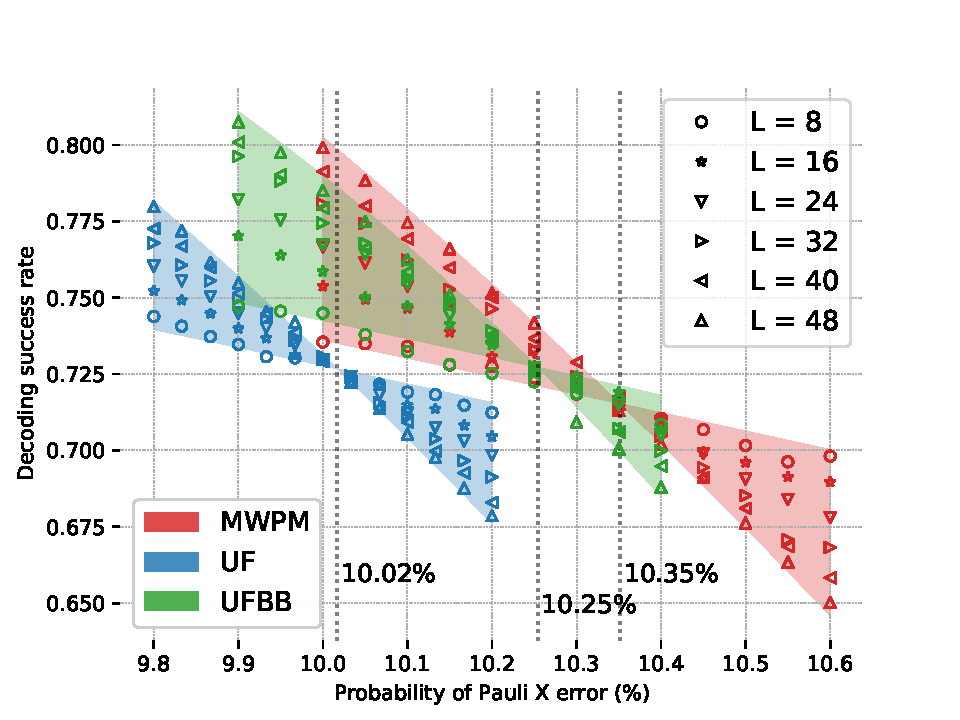
\includegraphics[width=\textwidth]{threshold.pdf}
    \caption{Decoder success rate and threshold.}\label{fig4}
\end{minipage}%
\begin{minipage}{.5\textwidth}
  \centering
    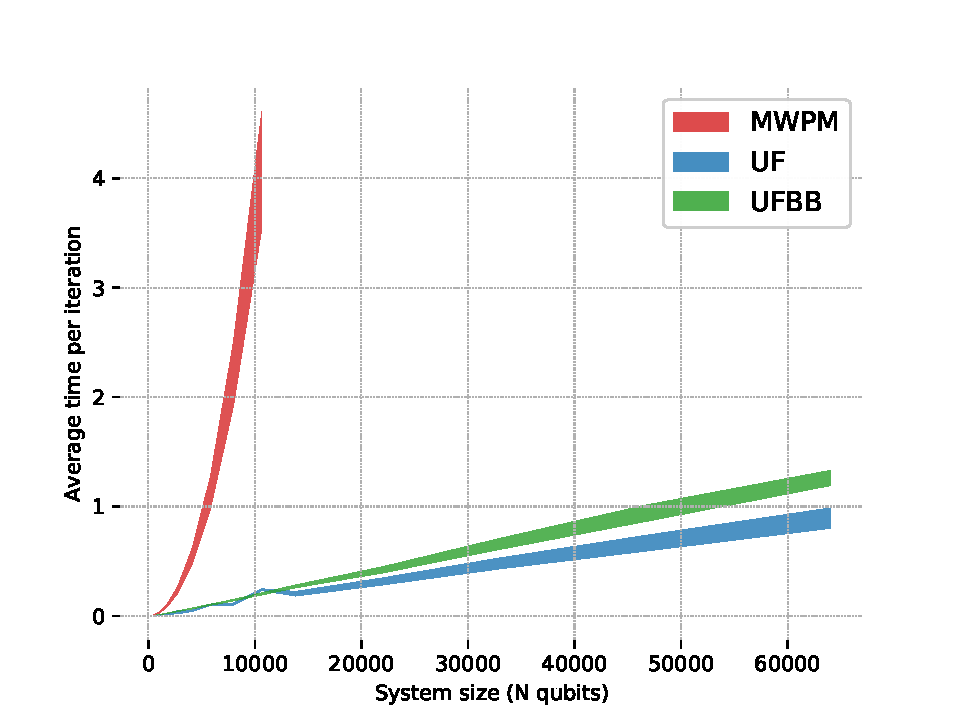
\includegraphics[width=\textwidth]{time.pdf}
    \caption{Decoder performance in computation time.}\label{fig5}
\end{minipage}
\end{figure}
\end{document} 